\documentclass[a4paper,10pt]{article}
\usepackage{float} % Add this line in your preamble
\usepackage{fancyhdr}
\usepackage{graphicx}
\usepackage{geometry}
\geometry{a4paper, left=2cm, right=2cm, top=1.5cm, bottom=3cm }
\usepackage{caption}
\usepackage{subcaption}
\usepackage{hyperref}
\usepackage{natbib}

\usepackage{etoolbox,fancyhdr,xcolor}
\newcommand{\headrulecolor}[1]{\patchcmd{\headrule}{\hrule}{\color{#1}\hrule}{}{}}
\newcommand{\footrulecolor}[1]{\patchcmd{\footrule}{\hrule}{\color{#1}\hrule}{}{}}
\renewcommand{\headrulewidth}{1pt}
\headrulecolor{red!100}%
\renewcommand{\footrulewidth}{1pt}
\footrulecolor{red!100}%

\fancyhf{}
\fancyhead[R]{\includegraphics[width=0.07\textwidth]{figures/UIC.jpg}}

\fancyfoot[L]{Project: Career Crafters}
\fancyfoot[C]{College of Engineering, Computer Science}
\fancyfoot[R]{\thepage}

\setlength{\headheight}{15mm}
\pagestyle{fancy}

\bibliographystyle{apalike}

\usepackage{times}
\begin{document}

\noindent 
\begin{center}
\textbf{{\Large CAREER CRAFTERS}} \\
\end{center}

\noindent 
\textbf{Authors: Saurav Joshi, Venkata Sesha Phani Vakicherla, Shahbaz Syed, Usha Pulivarthi, Venkata Rama Surya Sesha Siva Kumar Pidaparthi} \textit{University of Illinois, Chicago, IL}
\\

\noindent 
\textbf{ABSTRACT: } The job search process is daunting due to the vast number of online opportunities. To simplify this process, our team developed Career Crafters, a web application that tells job seekers how closely their skills match a job and actively recommends the best job matches based on their resumes. This report details our approach, combining data cleaning, machine learning techniques, and statistical analyses to provide highly personalized job recommendations, proving a valuable tool for job seekers.

\noindent 
\textbf{KEYWORDS:} Job Matching, Machine Learning, Recommendation Systems, Data Preprocessing, Natural Language Processing, Interactive Web Application. \\
\noindent 
\textbf{NOTE:} Please use any Document Viewer such as Acrobat or Document Viewer (Linux) that will correctly show the links for the Figures highlighted. Opening the PDF in the browser may not render the complete report functionality. 
\section{INTRODUCTION}

In today’s job market, finding the right job is often as challenging as getting it. While existing job search tools focus on indicating how well a candidate's qualifications match a job listing, they fall short in actively guiding users to their best matches. Career Crafters addresses this gap by offering a more proactive solution. Our system uses advanced machine learning to analyze job postings and candidate resumes, ensuring job seekers get recommendations that are close matches and the best possible options for their skills and experiences. This report will discuss how Career Crafters was built, from initial data handling to the deployment of personalized job recommendations, highlighting its advantages in helping candidates efficiently find suitable jobs.

\textbf{Github Project Link: } \hyperlink{https://github.com/sauravjoshi/Career-Crafters}{https://github.com/sauravjoshi/Career-Crafters}

% \subsection{Secondary Heading or Sub-headings}

% Here we have a sub-heading. There is no blank line after the sub-heading. You can have one level of subheadings but not a third i.e. you cannot have Section 1.1.1 as a subheading.

% \begin{itemize}
%     \item If you want to list bullet points you can do so;
%     \item This is the second point;
%     \item This is a third bullet point;
%     \item A fourth bullet point;
%     \item But you can.
% \end{itemize}   

% After a list you must leave a single blank line and remember to add the indent if you are starting a new paragraph.

% \subsection{Another sub-heading}

% You can have as many sub-headings in a section as you want to. Note that sub-headings have a 6pt spacing after them rather than a blank line but they are preceded by a blank line. The number of sections and sub-sections is up to you, as are the titles of each of them and this will be driven by the content of your report.

\section{DATA Processing}

\subsection{Data Collection}

    \subsubsection{Data Description}
    The Career Crafters application utilizes a comprehensive dataset of 32641 job postings, sourced from Kaggle and merged to form a consolidated database suitable for analysis. The data comprises 11 attributes such as Job Title, Company Name, Job Location, and more, all essential for developing accurate job recommendations.

    \subsubsection{Data Acquisition}
    \begin{itemize}
        \item \textbf{Master Data:} The data was acquired from Kaggle from different sources and merged based on relevant features to create a master set. \hyperlink{https://drive.google.com/file/d/12r3pCPnpawmdEmWB34k7UO1IjS2t4o34/view?usp=sharing}{https://drive.google.com/file/d/12r3pCPnpawmdEmWB34k7UO1IjS2t4o34/view?usp=sharing}
        \item \textbf{Software Engineer:} \hyperlink{https://www.kaggle.com/datasets/asaniczka/software-engineer-job-postings-linkedin}{https://www.kaggle.com/datasets/asaniczka/software-engineer-job-postings-linkedin}
        \item \textbf{Data Engineer:} \hyperlink{https://www.kaggle.com/datasets/asaniczka/linkedin-data-engineer-job-postings}{https://www.kaggle.com/datasets/asaniczka/linkedin-data-engineer-job-postings}
        \item \textbf{Data Analyst:} \hyperlink{https://www.kaggle.com/datasets/asaniczka/data-analyst-job-postings}{https://www.kaggle.com/datasets/asaniczka/data-analyst-job-postings}
        \item \textbf{Data Scientist:} \hyperlink{https://www.kaggle.com/datasets/asaniczka/data-scientist-linkedin-job-postings}{https://www.kaggle.com/datasets/asaniczka/data-scientist-linkedin-job-postings}
    \end{itemize}

    
    \subsubsection{Column Types and Data Characteristics}
        \begin{itemize}
        \item job\_title, company, job\_location, job\_link, first\_seen, search\_city, search\_country, job level, job\_type, job\_summary, job\_skills: All of these columns were string value. 
        \item First Seen: This column is Datetime, indicating when the job was first posted or collected.
        \item Derived Numerical Data: Post-processing, geo-coordinates were derived from the 'job\_location' text to facilitate spatial analysis.
    \end{itemize}   

\subsection{Data Wrangling}
    \subsubsection{Cleaning and Pre-Processing}
    Initial data cleaning involved string and list handling, where all attributes were cleansed to remove irrelevant characters and spaces, ensuring clean and usable text for analysis. Specifically, the `job\_summary` and `job\_skills` attributes, which had 411 and 1273 NA entries, respectively, were removed to maintain the integrity of the dataset, as imputing them or deriving them was not feasible.

    \subsubsection{Irregularities Handling}
        \begin{itemize}
        \item  Since the source data was scraped from LinkedIn, it was free-flow data. There were irregularities present in the job\_title such as Sr. Data Engineer, and Senior Data Engineer is effectively the same. Also, the job titles Senior Data Engineer, Public Company, and Senior Data Engineer are effectively the same. 
        \item Also, the job\_locations were not in a set format. This feature was also important to us for geospatial analysis of job distribution. There were some job postings without the proper address present. Also, since we had data from countries such as the UK, Australia, and Canada, having a uniform format was even more difficult.
        \item  Custom scripts were written specifically for these tasks that cater to the variance in these data and extract relevant information.
    \end{itemize}
    
    \subsubsection{Text Preprocessing (done over job\_skills\_summary)}
    \begin{itemize}
        \item \textbf{Tokenization and Normalization:} Job descriptions and skills were broken into tokens and normalized to lowercase to standardize the data.
        \item \textbf{Stop Words Removal:} Common stop words were removed to emphasize more significant terms relevant to job skills.
        \item \textbf{Punctuation Handling:} Punctuation marks were removed as they can interfere with text processing tasks like vectorization.
        \item \textbf{Part-of-Speech (POS) Tagging:} Words were tagged according to their parts of speech (e.g., noun, verb, adjective). We extracted clean POS from the initially tagged POS token by removing tokens with only 1 character. This gives us the final cleaned token. Certain specific tokens are also removed such as "company", "description", "title", "job", and "skills", as these are junk for a job\_description field. 
        \item \textbf{Lemmatization:} Words were reduced to their base form, aiding in uniformity and effectiveness in matching processes. Finally, lemmatization over the cleaned tokens are joined back to form the final processed job\_description string.
        \item \textbf{Vectorization:} Finally, the text was converted into a numeric format using vectorization techniques to feed textual data into machine learning algorithms.
    \end{itemize}
    
    \subsubsection{Feature Engineering}
    \begin{itemize}
        \item \textbf{Geo Code Retrieval:} After handling the above irregularities, geo-coordinates for each job posting were retrieved once standardized. This enabled precise geospatial analysis of job distribution, facilitating insights into regional employment trends and opportunities.
        \item \textbf{Interpolating job\_skills to job\_desc:} To consolidate and enhance the information available for our recommendation model, 'job\_skills' were combined with 'job\_summary' to create a new column called 'job\_skills\_summary.' This column integrates all critical skill-related information with the job descriptions, providing a unified data point that enhances the effectiveness of our job-matching algorithms by ensuring a comprehensive dataset for analysis.
    \end{itemize}
    
\section{EDA}
    
 \subsection{Heatmap of Job Locations}

      Figure \ref{fig_heatmap} shows us the job locations present across different countries. The jobs seem to be more concentrated in the West \& Mid-West of America than in the East; almost the entirety of Australia towards the East coast, mostly in London, Manchester, and Birmingham in the UK, and interestingly, almost every job in Canada comes with a location at a closer proximity with the US such as at Vancouver and Montreal. This visualization, in turn, gives rise to knowing what jobs are prevalent in which regions.

    \begin{figure}[ht]
    \centering
    \includegraphics[height=6.6cm]{figures/HeatMap.png}
    \caption{HeatMap for Job distribution. Visualization 1: Saurav Joshi}
    \label{fig_heatmap}
    \end{figure}


 \subsection{Dominant jobs based on cities}
      Figure \ref{fig_dominant_jobs} shows us the job locations that are present across different countries. The concentration of points illustrates the relative number of jobs in each region, visually representing job availability and market demand. The clusters of job points may correlate with economic centers and tech hubs, suggesting where certain industries are thriving. This allows candidates to target specific cities with more job postings per their required job titles.

    \begin{figure}[ht]
    \centering
    \includegraphics[height=6.6cm]{figures/dominant.png}
    \caption{Dominant job based on locations. Visualization 2: Saurav Joshi}
    \label{fig_dominant_jobs}
    \end{figure}

 \subsection{Job Postings and Resume in 2D t-SNE Space}
      Figure \ref{fig_tsne} shows us resume vs recommendation vs non-recommended jobs in a two-dimensional t-SNE space. The cluster of blue dots near the 'X' suggests that the top recommendations are closely aligned with the resume's features.

    \begin{figure}[ht]
    \centering
    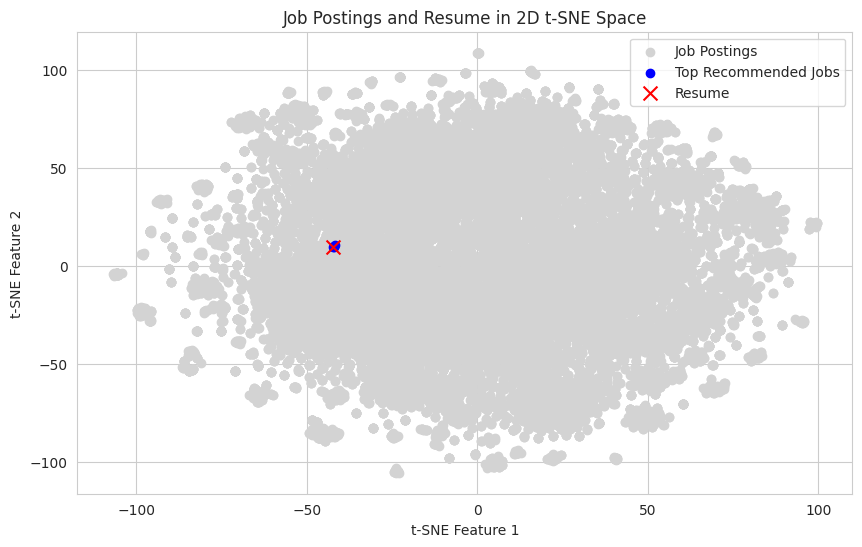
\includegraphics[height=6.6cm]{figures/17.png}
    \caption{Job Postings (Entire Corpus) VS Recommended Jobs vs Resume. Visualization 3: Saurav Joshi}
    \label{fig_tsne}
    \end{figure}
    

\subsection{Resume specific Top skills for recommended jobs - Venkata Sesha Phani Vakicherla (1)}

Figure \ref{fig_phani_1} shows a visualization of the top skills extracted from candidates' resumes and how these skills align with those required by jobs recommended by our system. This analysis helps demonstrate our matching algorithm's effectiveness in identifying and recommending positions that best fit the candidates' skill sets.

    \begin{figure}[ht]
    \centering
    \includegraphics[height=6.6cm]{figures/Vis_1_Phani.png}
    \caption{Resume specific Top skills for recommended jobs. Visualization 1: Phani}
    \label{fig_phani_1}
    \end{figure}

\subsection{Distribution of word counts in the job description- Venkata Sesha Phani Vakicherla (2)}
Figure \ref{fig_phani_2} shows the distribution of tokens in the text corpus. It is important to note the presence of outliers within our data—specifically, job descriptions that contain over 800 tokens. These outliers have not been removed or truncated despite their deviation from the norm. The rationale behind this decision is based on the potential value they hold. These comprehensive summaries are likely to be rich in information, providing depth that could enhance our model.

\begin{figure}[H]
    \centering
    \begin{minipage}{0.5\textwidth}
        \centering
        \includegraphics[height=6cm]{figures/Phani.png}
        \caption{Distribution of word counts in the job description. Visualization 2: Phani}
        \label{fig_phani_2}
    \end{minipage}%
    \hfill
    \begin{minipage}{0.48\textwidth}
        \centering
        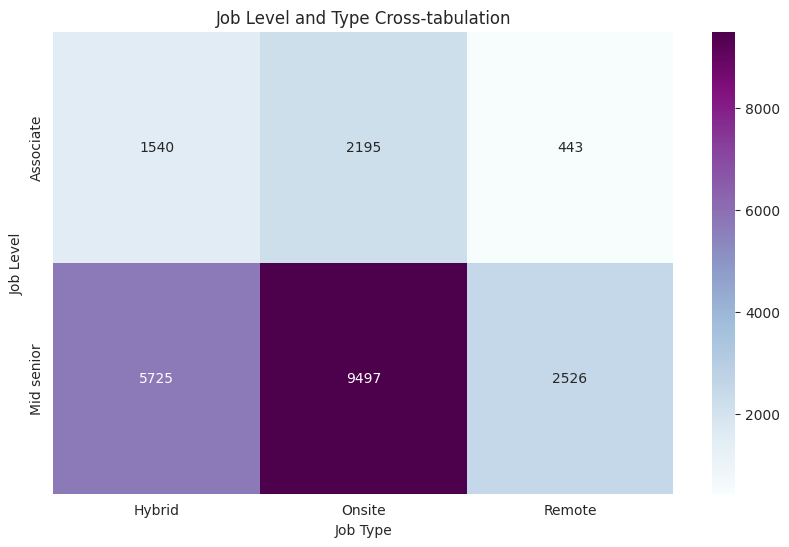
\includegraphics[height=6cm]{figures/11.png}
        \caption{Cross-tabulation of job levels against job types. Visualization 3: Phani}
        \label{fig_phani_3}
    \end{minipage}
\end{figure}

\subsection{Job Level and Type Cross-tabulation - Venkata Sesha Phani Vakicherla (3)}
Figure \ref{fig_phani_3} visualizes a cross-tabulation of job levels against job types. - Mid-senior level roles dominate, especially in the onsite category, indicating a mature job market.
Associate roles are fewer compared, with hybrid roles outnumbering remote opportunities at this level. This data could inform job seekers about the most prevalent job types at different career stages.


\subsection{Top Job Titles from Job Postings}
Figure \ref{fig_shabaz1} provides a summary of the most demanded job titles based on the count of job postings. It highlights the importance of technology and data-related roles. Senior Software Engineer and Software Engineer are the most frequently advertised positions. This suggests a strong job market and high demand for professionals with software engineering skills.

    \begin{figure}[ht]
    \centering
    \includegraphics[height=6cm]{figures/Shahbaz1.png}
    \caption{Top 20 job titles from job postings. Visualization 1: Shahbaz}
    \label{fig_shabaz1}
    \end{figure}

\subsection{Word Cloud for Job Skills of Top Jobs}
Figure \ref{fig_shabaz2} displays a word cloud related to job skills for the top 5 types of jobs. This representation emphasizes the importance of the skills mentioned in job postings or descriptions. Words with larger sizes indicate a higher demand for those particular skills. Key skills like "Software," "Development," "Engineering," "Data," "System," "SQL," "Python," and "AWS" stand out as important, suggesting they are highly sought after in the job market. Skills associated with data handling like "Data Modeling," "Data Warehouse," and "Machine Learning" are also significant, reflecting the importance of data management and analytics. 

    \begin{figure}[ht]
    \centering
    \includegraphics[height=6cm]{figures/Shahbaz2.png}
    \caption{Word Cloud for Job Skills for Top 5 Jobs Titles. Visualization 2: Shahbaz}
    \label{fig_shabaz2}
    \end{figure}

\subsection{Top Skills Demand by Job Type and Location}
Figure \ref{fig_venkata1} visualizes presents the demand for various job skills across key global cities, categorizing roles into Hybrid, Onsite, and Remote. It reveals a notable preference for remote jobs in cities like New York and San Francisco, while onsite work remains prevalent in Chicago and London.
This visualization is a strategic guide for job seekers and companies to understand and adapt to evolving employment trends.

    \begin{figure}[ht]
    \centering
    \includegraphics[width=0.5\textwidth,height=6cm]{figures/joblocloc.png}
    \caption{Cross-tabulation of job levels against job types. Visualization 1: Venkata}
    \label{fig_venkata1}
    \end{figure}

\subsection{Job Type Preferences and Job Search by Country}
Figures \ref{fig_venkata2} below depict bar graphs from a numerical perspective. The first graph shows job type preferences, with the x-axis representing the quantity and the y-axis listing job types: Remote, Onsite, and Hybrid. Onsite jobs are the most popular, followed by hybrid jobs, with remote jobs being the least preferred. The second graph illustrates job searches or applications by country, featuring the United States, United Kingdom, Canada, and Australia on the y-axis. It highlights that the United States has the highest number of searches or applications, significantly more than the United Kingdom, Canada, and Australia, which follow in descending order. These visualizations are useful for analyzing trends in job preferences and the geographical distribution of job seekers.

    \begin{figure}[ht]
    \centering
    \includegraphics[height=6cm]{figures/1212.png}
    \caption{Job Type Preferences and Job Search by Country. Visualization 2: Venkata}
    \label{fig_venkata2}
    \end{figure}

\subsection{Top 10 Job Skills}
Figure \ref{fig_top_10} ranks the top 10 normalized job skills in frequency, with 'SQL' and 'Python' leading the chart, indicating their high demand in the tech industry. Skills in 'data analysis' and 'java' are also prevalent, while 'communication' skills are emphasized as essential. This information is crucial for job seekers prioritizing their learning and development focus areas.

    \begin{figure}[ht]
    \centering
    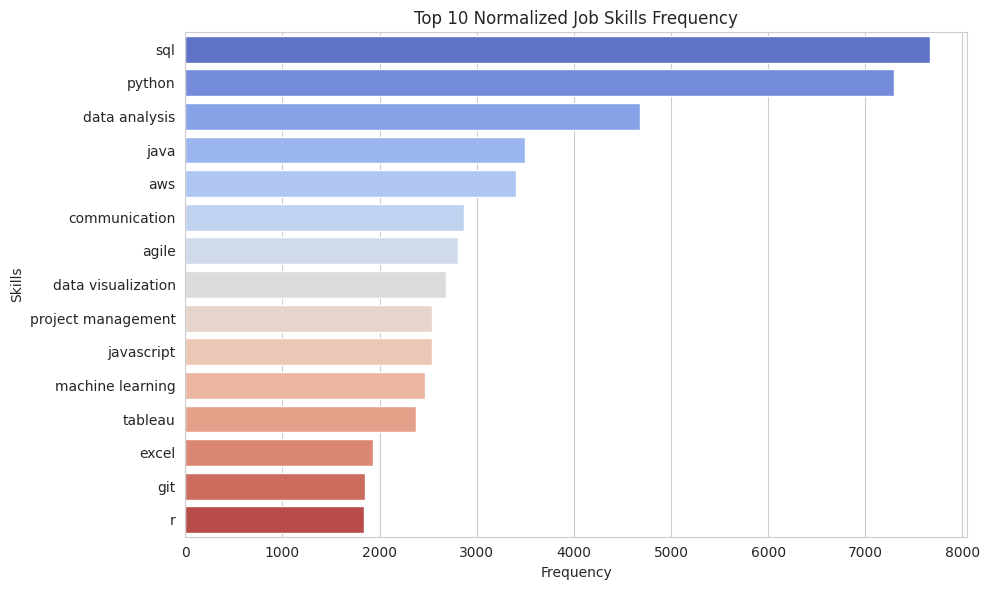
\includegraphics[height=6cm]{figures/13.png}
    \caption{Bar chart ranks the top 10 normalized job skills in frequency. Visualization 1: Usha}
    \label{fig_top_10}
    \end{figure}
    
\subsection{Word cloud for job skills}
Figure \ref{fig_job_skills_word_cloud} focuses on key skills relevant to the job market, with terms like 'data analysis,' 'machine learning,' 'project management,' and 'software development' being especially prominent.This suggests a high demand for these skills across various industries in general.The graphic serves as a visual guide for individuals looking to refine their expertise to align with market needs.

    \begin{figure}[ht]
    \centering
    \includegraphics[height=6cm]{figures/usha2.png}
    \caption{Word cloud for job skills. Visualization 2: Usha}
    \label{fig_job_skills_word_cloud}
    \end{figure}


\section{Machine Learning and Statistical Analysis}

Each member of the Career Crafters team utilized at least one advanced machine learning or statistical analysis technique to analyze the data and extract meaningful insights:

\subsection{Saurav Joshi: GloVe Embeddings, Cosine Similarity Match, and K-Nearest Neighbors}
\textbf{Technique Used:} GloVe Embedding\\
\textbf{Description:} Implemented GloVe to generate word embeddings by aggregating global word-word co-occurrence matrix from the job postings. The GloVe model was trained over 4 epochs with 100 Dim, 5 Window, and 4 Threads. The rationale behind using GloVe in addition to Word2Vec was that Word2Vec works in a local context, whereas Glove works in a global context. This global perspective can lead to more robust embeddings, capturing relationships that Word2Vec might miss due to its local approach.\\
\textbf{Inferences:} This technique facilitated the vectorization of tokens into meaningful numerical representations, embedding semantically rich information. These embeddings enabled more sophisticated recommendation mechanisms, enhancing the system's capability to match job seekers with roles requiring similar skills despite variations in job titles.

\textbf{Additional Technique: Cosine Similarity Match}\\
\textbf{Description:} Utilized cosine similarity to measure the distance between the vectorized features of job postings and candidate resumes. This method assesses the cosine of the angle between two vectors in a multi-dimensional space, providing a similarity score that is crucial for effective job matching.\\
\textbf{Inferences:} This similarity metric has proven essential in filtering and ranking job postings that are most relevant to the candidate's skills and experiences, significantly enhancing the precision of our recommendations.

\textbf{Additional Technique: K-Nearest Neighbors (K-NN)}\\
\textbf{Description:} Applied the K-NN algorithm to classify job postings based on the closest feature vectors derived from resumes. K-NN focuses on a defined neighborhood, which can be helpful when a context-specific analysis is needed. This allows for finding a cluster of similar items or data points rather than just measuring similarity to a single point.
\\
\textbf{Inferences:} K-NN allowed to effectively narrow the list of potential job matches to those that best fit the candidates' qualifications and preferences, giving better results than just cosine-similarity-based top results.

\textbf{Additional Visualization: Job Recommendations Comparison based on KNN Match distance: }\\
\textbf{Description:} This figure \ref{fig_comparison} displays top Match Distances from the resume on different embeddings, providing a snapshot of the recommendation system’s output based on the candidate's resume and the embedding technique associated.\\
\textbf{Inferences:} This clearly shows that Word2Vec and GloVe outshine naive vectorization techniques, with GloVe performing best. This was later verified by a custom recommendation result analysis. 

 \begin{figure}[ht]
    \centering
    \includegraphics[height=5.5cm]{figures/Comparison.png}
    \caption{KNN - Match Distances - Visualization 4: Saurav Joshi}
    \label{fig_comparison}
    \end{figure}
\subsection{Venkata Sesha Phani Vakicherla: Word2Vec Embedding, Visualizations of Top Job Matches, Recommended vs Non-Recommended Jobs}
\textbf{Technique Used:} Word2Vec Embedding\\
\textbf{Description:} Manually trained a Word2Vec model to create word embeddings that capture semantic meanings of the skills and job titles within the dataset. The model settings included 100 dimensions, a window size of 5, and a minimum count of 2, running on 4 threads.\\
\textbf{Inferences:} The embeddings helped understand the relationship between different skills and job titles, enabling the recommendation system to suggest jobs that closely match candidates' profiles based on semantic similarity.

\textbf{Additional Visualization: 3D Scatter Plot: Resume vs Recommended Jobs vs Non-Recommended Jobs}\\
\textbf{Description:} This 3D scatter plot \ref{fig_scat_plot} visualizes the distinction between recommended (blue) and non-recommended (gray) job postings relative to a candidate’s resume within a compressed feature space. \\
\textbf{Inferences:} The proximity of blue points to the resume indicates accurate recommendations by the system, while the dispersed gray points reflect lesser relevance to the candidate's profile.

    \begin{figure}[ht]
    \centering
    \includegraphics[height=6.5cm]{figures/Phani_3D_ScatterPlot.png}
    \caption{(System Recommended) Resume vs Recommended Jobs. Visualization 4: Phani}
    \label{fig_scat_plot}
    \end{figure}

\textbf{Additional Visualization: Top Job Matches based on Resume}\\
\textbf{Description:} This figure \ref{fig_table} displays top job matches providing a snapshot of the recommendation system’s output based on candidates resume.\\
\textbf{Inferences:} The varied job types and levels across different cities suggest the system's capability to personalize job recommendations effectively, catering to diverse candidate profiles and preferences.

 \begin{figure}[ht]
    \centering
    \includegraphics[height=6cm]{figures/Phani_Table.png}
    \caption{Top Job Matches based on Resume. Visualization 5: Phani}
    \label{fig_table}
    \end{figure}

\subsection{Shahbaz: Resume Parser}
\textbf{Technique: Resume Parser}\\
\textbf{Description:} Used Python Flask, Pyreparser for resume parsing \\
\textbf{Inferences:} Pyreparser is built upon Python and utilizes natural language processing (NLP) to extract information from resumes. It can help automate the task of reading and extracting data such as personal information, skills, experience, and education from many resumes.

\textbf{Additional Visualization: Comparison of Job Recommendations by Cosine Similarity}\\
\textbf{Description:} This 3D scatter plot \ref{fig_shahbaz3} The visualization is a scatter plot titled "Comparison of Job Recommendations by Cosine Similarity," which compares the performance of four different text analysis methods: TF-IDF, Count Vectorizer, Word2Vec, and GloVe.  \\
\textbf{Inferences:} Word2Vec and GloVe outperform TF-IDF and Count Vectorizer significantly in terms of cosine similarity scores, suggesting that these methods are more effective in capturing semantic similarities between job descriptions for recommendation purposes.

    \begin{figure}[ht]
    \centering
    \includegraphics[height=6.5cm]{figures/Shahbaz3.png}
    \caption{Comparison of Job Recommendations by Cosine Similarity. Visualisation 3 : Shahbaz}
    \label{fig_shahbaz3}
    \end{figure}




\subsection{Usha: TF-IDF Vectorization, Visualization of Top 10 skills for top job titles}
\textbf{Technique Used:} TF-IDF Vectorization\\
\textbf{Description:} Used TF-IDF to transform text data into a vectorized format, weighting terms based on their importance to a document relative to the entire dataset.\\
\textbf{Inferences:} The analysis identified key terms and skills critical in different industries, which helped tailor job recommendations to specific sectoral needs.

\textbf{Additional Technique: Web Application Development}\\
\textbf{Description:} React Typescript, Tailwind CSS, react-plotly for charts \\
\textbf{Inferences:} Worked on the frontend development for the interactive web application of career crafters.


 \textbf{Additional Visualization: Top 10 Skills for Top Job Titles}\\
 \textbf{Description:} This visualization\ref{fig_usha} helps us know the most common skills required in jobs. This can help candidates align themselves with these skills based on the job they are looking for. Also, it can be seen as learning Python, and SQL has the best advantage as it is present across job titles..\\
\textbf{Inferences:} The visualization highlights Python and SQL as essential skills across multiple top job titles, underscoring their importance in the job market. This trend suggests that candidates proficient in these skills are better positioned to meet the demands of key roles in technology and data-centric fields. As such, job seekers should consider prioritizing these skills to enhance their employability and align with industry requirements.

\begin{figure}[ht]
    \centering
    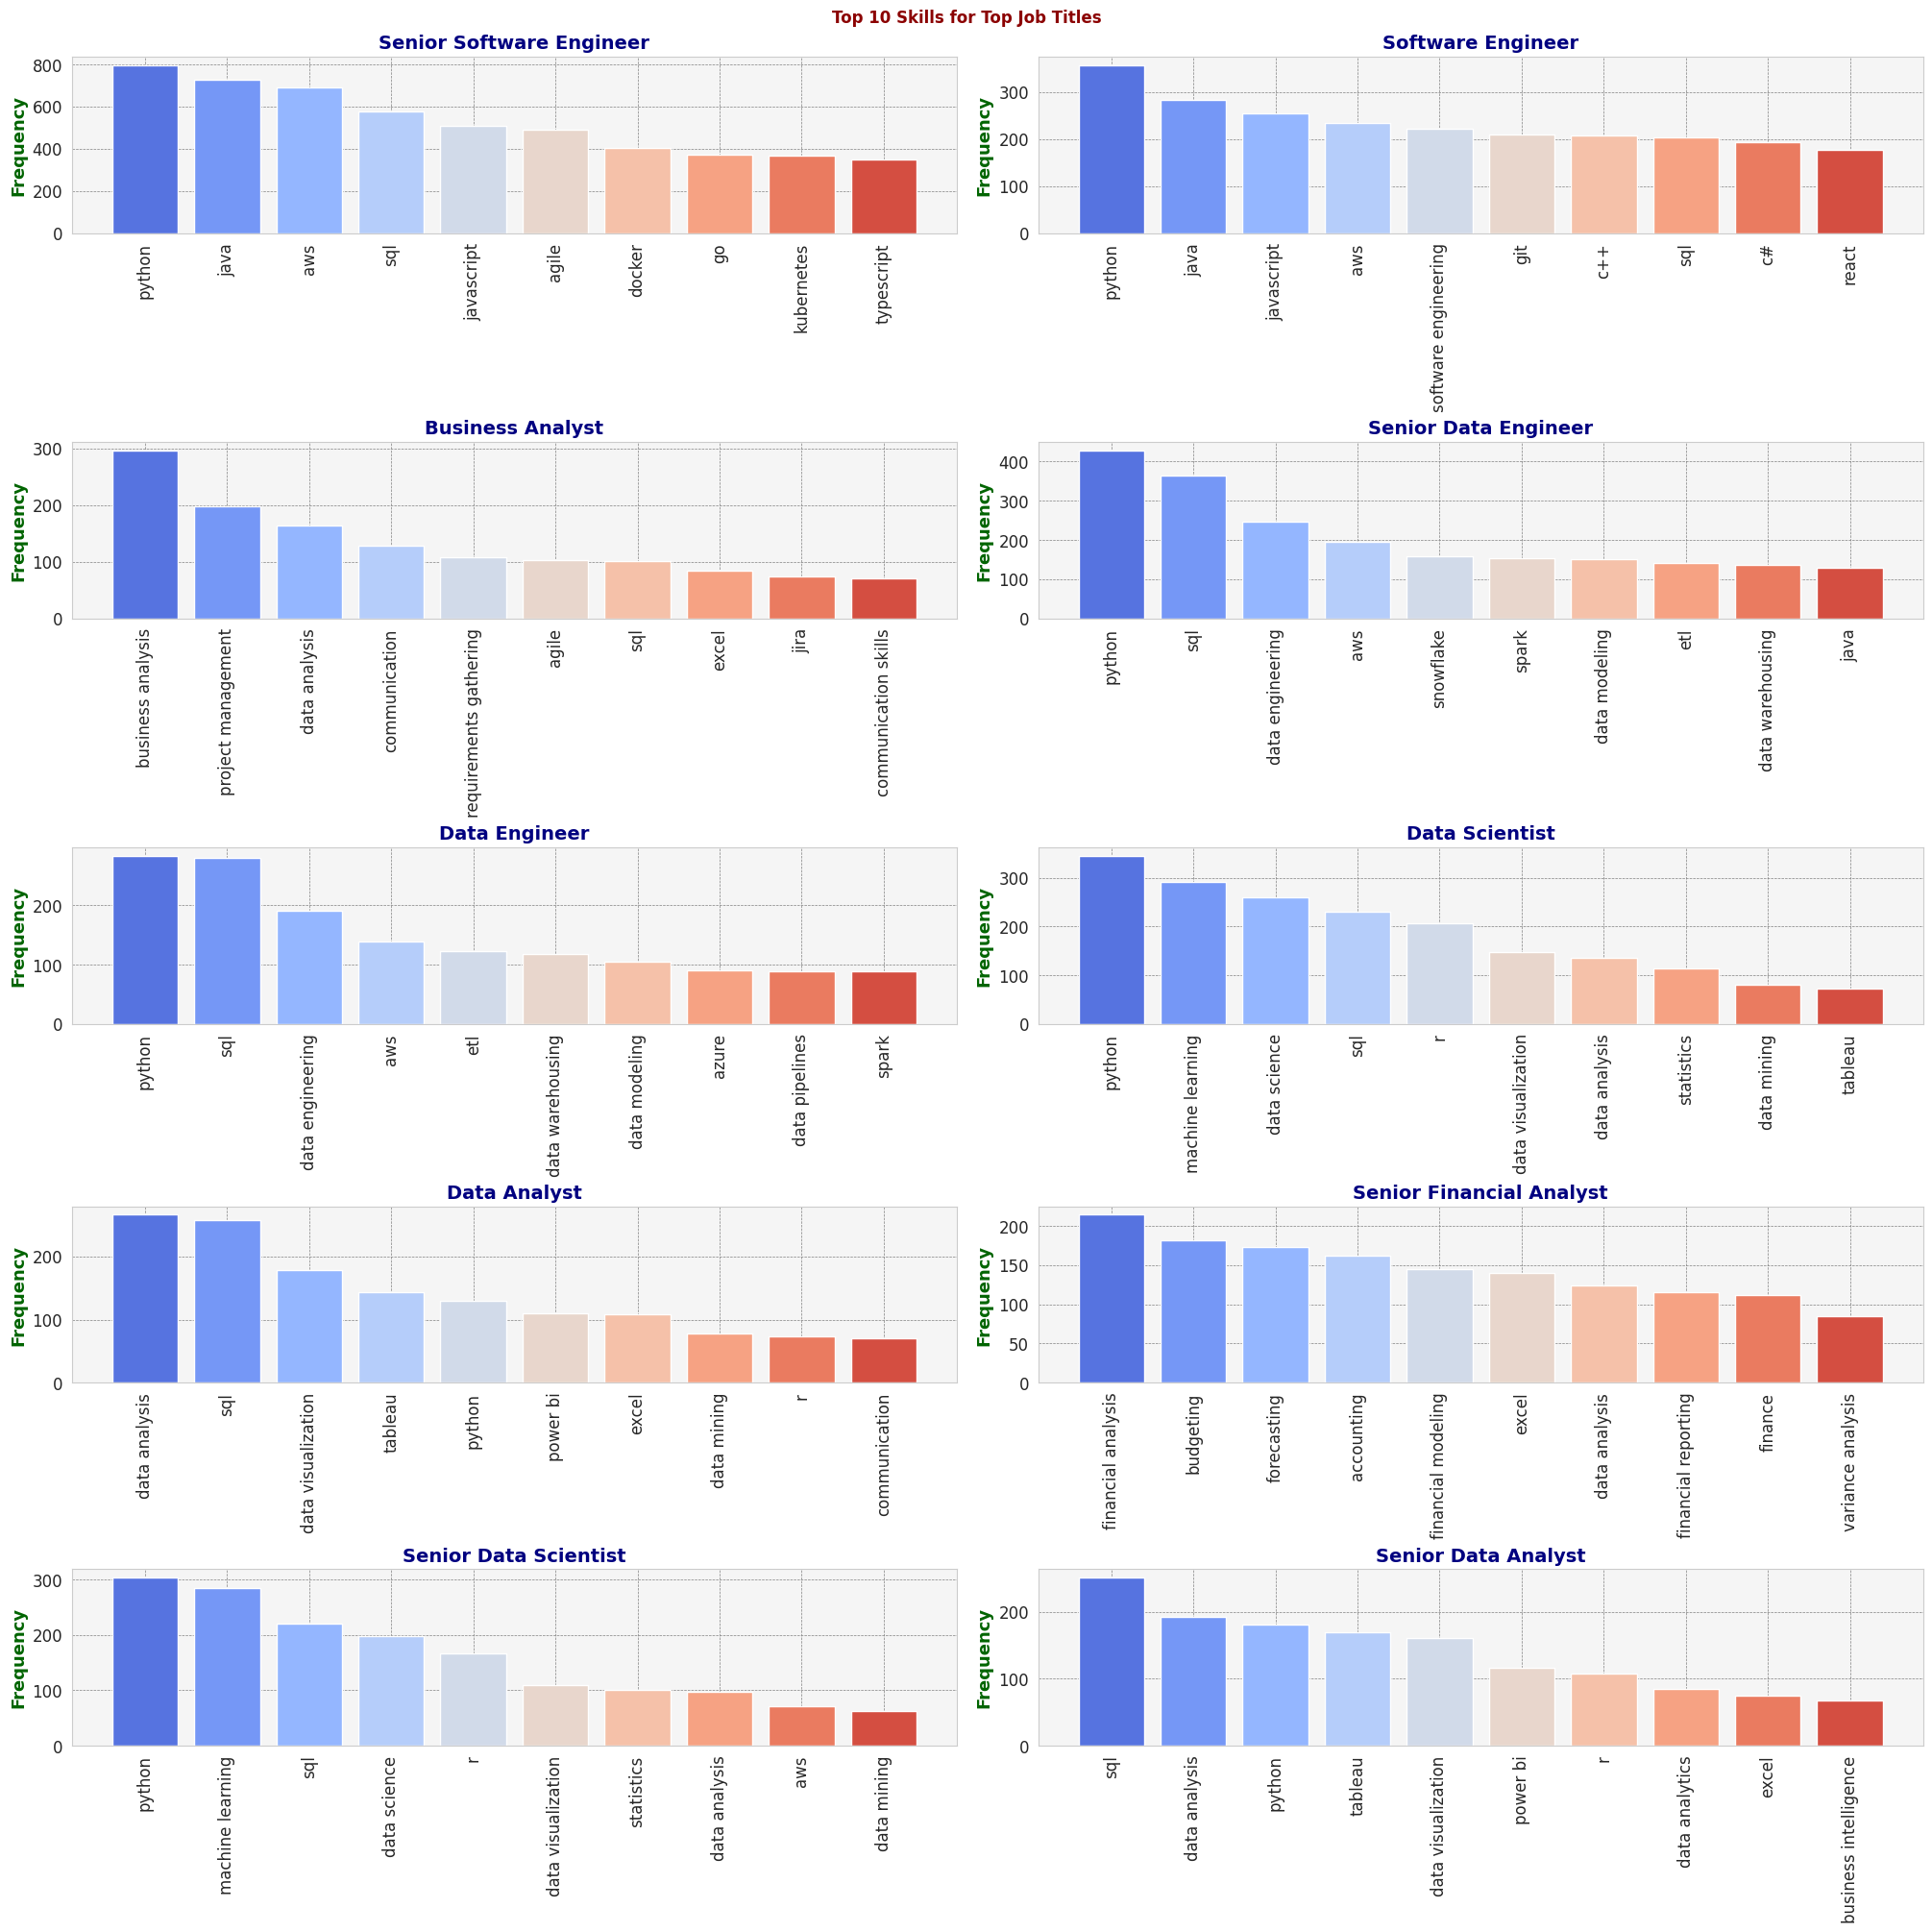
\includegraphics[width=0.6\textwidth,height=8cm]{figures/14.png}
    \caption{Top 10 Skills for Top Job Titles. Visualization 3: Usha}
    \label{fig_usha}
    \end{figure}  
    
\subsection{Venkat: CountVectorizer}
\textbf{Technique Used:} CountVectorizer\\
\textbf{Description:} Employed CountVectorizer as a baseline to convert text data into a matrix of token counts, allowing comparison against more sophisticated models.\\
\textbf{Inferences:} While basic, this approach provided a foundational understanding of the frequency of various job-related terms, which assisted in the initial filtering and categorization of job postings.

\textbf{Additional Visualization: Geographical Distribution of Remote vs Onsite Jobs}\\
\textbf{Description:} This map \ref{GeoDi} visually differentiates between remote, onsite, and hybrid jobs based on location, highlighting regional preferences or necessities for job types. It's a tool for understanding the job market's geographical nuances, offering insights for job seekers, companies, and analysts.\\
\textbf{Inferences:}
- Helps job seekers find areas with a high density of preferred job types.
- Aids companies in identifying regions with the workforce they need.
- Provides market insights for strategic decisions and trend analysis.

\begin{figure}[ht]
    \centering
    \includegraphics[width=1\textwidth,height=6cm]{figures/GeoDi.png}
    \caption{Geographical Distribution of Remote vs Onsite Jobs. Visualization 3: Venkata}
    \label{GeoDi}
    \end{figure}


\section{Results \& Future Work}

The recommendation engine and the accompanying web application form the core of the Career Crafters project's results. They ease job search by offering a personalized, data-driven service that is functional but also engaging and user-centric by using the system's ability to match job seekers with the right opportunities based on a nuanced understanding of their skills and job market trends.

 \begin{figure}[ht]
    \centering
    \includegraphics[height=4cm]{figures/Results.png}
    \caption{Final Results}
    \label{fig_results}
    \end{figure}

\begin{itemize}
    \item Total 7 Resumes considered for checking efficacy amongst top 5 recommendations for each embedding using K-NN.

    \item  Relevant Skills and Relevant Titles are matched using a Fuzzy String matching.
    \begin{itemize}
    	\item Skills with a partial\_ratio of greater than 80\%.
    	\item Titles with a partial\_ratio of greater than 90\%.
    \end{itemize}
\end{itemize}

\textbf{Embedding Techniques Comparison}:
\begin{itemize}
 \item A comparison of embedding techniques revealed that GloVe outperformed others with an 80\% match for relevant skills and an 85.71\% match for job titles. This high performance indicates a strong alignment between the job recommendations provided by the system and the candidates' profiles and preferences.

 \item Word2Vec also showed promising results, especially in matching relevant job titles with a match percentage of 82.85\%, indicating its effectiveness in capturing the context of job descriptions and titles.
\end{itemize}

\textbf{Analysis of Recommendation System}:
\begin{itemize}
 \item The system was tested with 7 resumes, evaluating the top 5 recommendations for each resume against various embeddings using the K-NN algorithm. This practical approach to testing helped fine-tune the recommendation engine for precision.

 \item The relevance of the matches was determined using a fuzzy string matching algorithm, with a partial ratio threshold set to ensure only the most appropriate recommendations were considered successful. Skills and titles meeting these criteria underscore the tailored nature of the job-matching process.

\end{itemize}

\subsection{Interactive Web Application}

A key outcome of the project is an interactive web application that showcases the recommendation engine in real-time operation. This user-friendly interface allows job seekers to experience firsthand the sophistication of the recommendation system. Users can submit their resumes through the web application and instantly receive job recommendations.

The web application's front end is built using React with TypeScript, styled with Tailwind CSS, and integrates react-plotly for dynamic data visualization. The back end is developed in Python using the Flask framework, with vector models for the recommendation engine stored in files to facilitate quick and efficient data processing.

The source code and additional documentation are available on GitHub at: \href{https://github.com/sauravjoshi/Career-Crafters}{https://github.com/sauravjoshi/Career-Crafters}. Demo available at: \url{https://www.youtube.com/watch?v=JDnYAXXDxpU}

\subsection{Limitations}
While Career Crafters has made significant strides in job matching, the following limitations are acknowledged:
\begin{itemize}
  \item The recommendation engine's adaptability to the complexities and nuances of varied job roles across different industries has room for enhancement.
  \item The system currently does not incorporate a real-time data syncing mechanism, which could potentially limit the reflection of immediate market changes.
\end{itemize}

\subsection{Recommendations for Further Work}
Based on the project's roadmap and current limitations, the following future work is proposed:
\begin{itemize}
  \item \textbf{Advanced BERT Embeddings:} Employ more sophisticated BERT embeddings to improve contextual understanding within job descriptions, increasing the precision of job matches.
  \item \textbf{Content-Based Clustering:} Investigate content-based clustering approaches for recommendations to effectively group similar jobs and candidate profiles, allowing for refined and tailored matches.
  \item \textbf{Continuous Data Ingestion:} Develop a pipeline for the continuous updating of the job postings corpus to maintain data relevance and accuracy.
  \item \textbf{Feedback Ingestion:} Integrate user feedback mechanisms into the system to capture user preferences and interactions, facilitating the personalization and continuous improvement of the recommendation algorithms.
\end{itemize}

\section*{Acknowledgments}

We express our deepest gratitude to Professor Saurav Medya for his invaluable guidance and continuous support throughout the duration of this project. His insights and expertise were instrumental in shaping the direction and success of our work. Special thanks to the teaching assistants, Peyman and Khushboo, whose assistance and dedication played a pivotal role in our research and development process. Their feedback and suggestions were greatly appreciated and contributed significantly to the refinement of the Career Crafters system.

We would also like to extend our thanks to the University of Illinois Chicago (UIC) for providing the resources and environment conducive to our academic and project pursuits. The support and opportunities offered by UIC have been essential to our learning and success.

\end{document}
